% --- Chart 1: Execution Time ---
\begin{figure}[!ht]
  \centering
  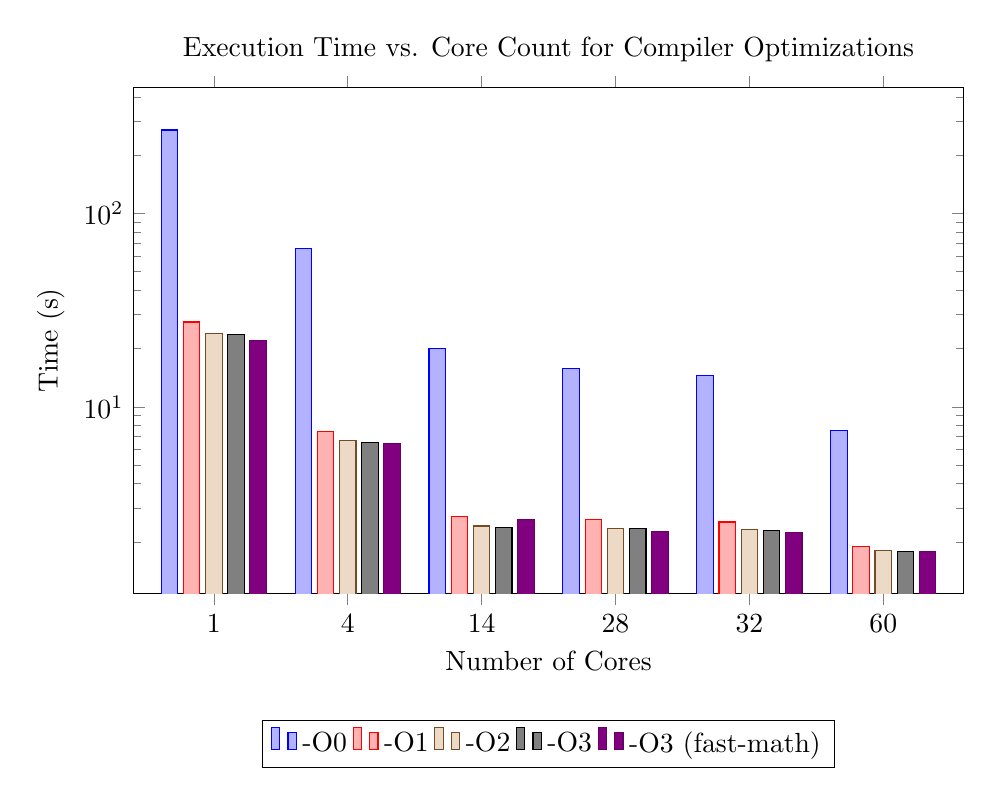
\begin{tikzpicture}
    \begin{axis}[
        title={Execution Time vs. Core Count for Compiler Optimizations},
        width=\textwidth,   
        height=8cm,         
        ybar,               
        ymode=log,          
        log basis y={10},
        enlarge x limits=0.12, 
        xlabel={Number of Cores},
        ylabel={Time (s)},
        symbolic x coords={1, 4, 14, 28, 32, 60},
        xtick=data, 
        bar width=6pt, 
        legend style={
          at={(0.5,-0.25)},
          anchor=north,
          legend columns=-1 
        },
        yticklabel style={
            /pgf/number format/fixed,
            /pgf/number format/precision=2
        },
    ]
    % Add a plot for each optimization flag. pgfplots groups them automatically.
    \addplot coordinates {(1, 270.06) (4, 66.066) (14, 19.9344) (28, 15.729) (32, 14.4472) (60, 7.5463)};
    \addplot coordinates {(1, 27.453) (4, 7.4351) (14, 2.7184) (28, 2.6043) (32, 2.5369) (60, 1.89955)};
    \addplot coordinates {(1, 24.02) (4, 6.67) (14, 2.42) (28, 2.36) (32, 2.33) (60, 1.80)};
    \addplot coordinates {(1, 23.5993) (4, 6.5605) (14, 2.3807) (28, 2.3382) (32, 2.3015) (60, 1.79288)};
    \addplot coordinates {(1, 22.054) (4, 6.478) (14, 2.62) (28, 2.2701) (32, 2.2368) (60, 1.79288)};

    \legend{-O0, -O1, -O2, -O3, -O3 (fast-math)}
    \end{axis}
  \end{tikzpicture}
  \caption[Execution time for multiple compiler flags]{Execution time (log scale) for various core counts and compiler flags.}
  \label{fig:time-chart}
\end{figure}

% --- Chart 2: Package Energy ---
\begin{figure}[!ht]
  \centering
  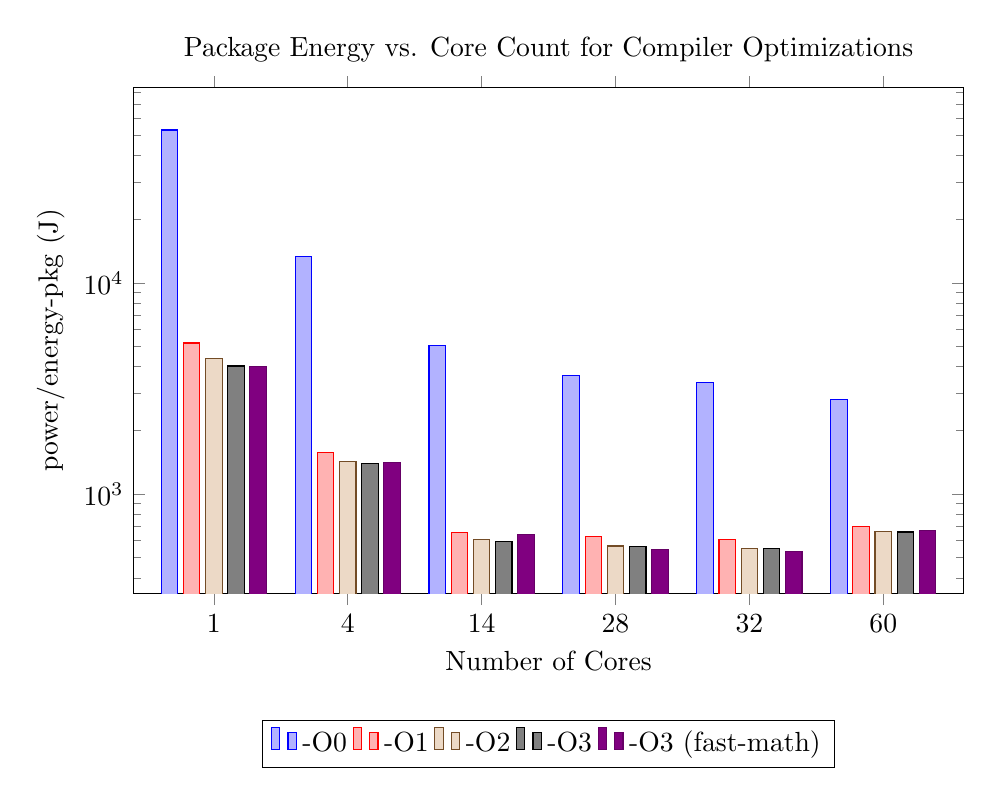
\begin{tikzpicture}
    \begin{axis}[
        title={Package Energy vs. Core Count for Compiler Optimizations},
        width=\textwidth,
        height=8cm,
        ybar,
        ymode=log,
        log basis y={10},
        enlarge x limits=0.12,
        xlabel={Number of Cores},
        ylabel={power/energy-pkg (J)},
        symbolic x coords={1, 4, 14, 28, 32, 60},
        xtick=data,
        bar width=6pt,
        legend style={
          at={(0.5,-0.25)},
          anchor=north,
          legend columns=-1
        },
        yticklabel style={
            /pgf/number format/fixed,
            /pgf/number format/precision=2
        },
    ]
    \addplot coordinates {(1, 52957.47) (4, 13379.59) (14, 5056.15) (28, 3650.43) (32, 3353.53) (60, 2794.03)};
    \addplot coordinates {(1, 5185.28) (4, 1564.51) (14, 658.46) (28, 627.89) (32, 606.52) (60, 698.96)};
    \addplot coordinates {(1, 4388.12) (4, 1417.01) (14, 606.58) (28, 565.83) (32, 552.98) (60, 661.76)};
    \addplot coordinates {(1, 4031.83) (4, 1386.60) (14, 595.29) (28, 561.59) (32, 548.83) (60, 659.31)};
    \addplot coordinates {(1, 4005.70) (4, 1414.08) (14, 639.00) (28, 547.56) (32, 535.22) (60, 671.51)};

    \legend{-O0, -O1, -O2, -O3, -O3 (fast-math)}
    \end{axis}
  \end{tikzpicture}
  \caption[Package consumption for multiple compiler flags]{Package energy consumption (log scale) for various core counts and compiler flags.}
  \label{fig:pkg-energy-chart}
\end{figure}

% --- Chart 3: RAM Energy ---
\begin{figure}[!ht]
  \centering
  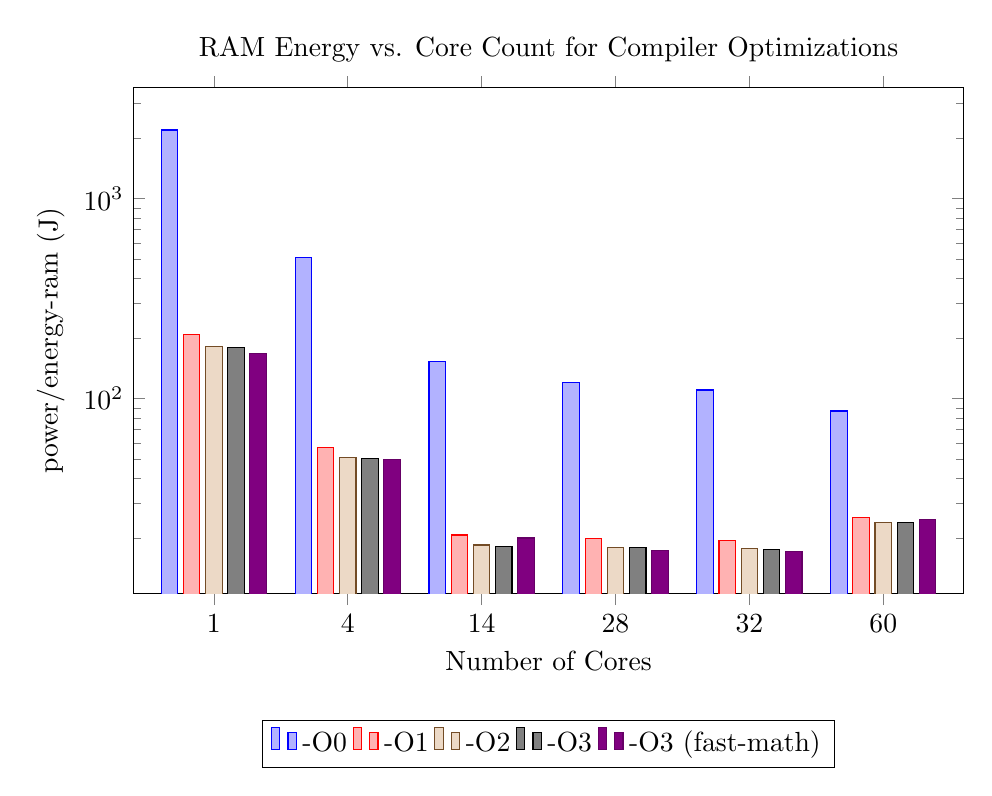
\begin{tikzpicture}
    \begin{axis}[
        title={RAM Energy vs. Core Count for Compiler Optimizations},
        width=\textwidth,
        height=8cm,
        ybar,
        ymode=log,
        log basis y={10},
        enlarge x limits=0.12,
        xlabel={Number of Cores},
        ylabel={power/energy-ram (J)},
        symbolic x coords={1, 4, 14, 28, 32, 60},
        xtick=data,
        bar width=6pt,
        legend style={
          at={(0.5,-0.25)},
          anchor=north,
          legend columns=-1
        },
        yticklabel style={
            /pgf/number format/fixed,
            /pgf/number format/precision=2
        },
    ]
    \addplot coordinates {(1, 2208.08) (4, 508.40) (14, 153.03) (28, 120.49) (32, 110.47) (60, 86.80)};
    \addplot coordinates {(1, 210.28) (4, 56.72) (14, 20.79) (28, 20.00) (32, 19.54) (60, 25.37)};
    \addplot coordinates {(1, 183.21) (4, 50.96) (14, 18.53) (28, 18.00) (32, 17.76) (60, 24.11)};
    \addplot coordinates {(1, 180.00) (4, 50.37) (14, 18.24) (28, 17.93) (32, 17.58) (60, 24.10)};
    \addplot coordinates {(1, 168.52) (4, 49.56) (14, 20.10) (28, 17.47) (32, 17.27) (60, 24.76)};

    \legend{-O0, -O1, -O2, -O3, -O3 (fast-math)}
    \end{axis}
  \end{tikzpicture}
  \caption[RAM consumption for multiple compiler flags]{RAM energy consumption (log scale) for various core counts and compiler flags.}
  \label{fig:ram-energy-chart}
\end{figure}